\originalchapter{8.05 作业8：相干、压缩与光场模式}
来源为Fall 2013 Assignment 8, 2013年11月2日发布, 11月8日15时截止. 第1--6题中文转述, 解答为\textbf{AI独立解答}; 第5题保留based on Sakurai 2.9署名, 依MIT实际完整题面独立解答. 基础相干态和两态动力学亦有本册独立章节支持.
\originalsection{第1题：位置和动量广义本征态}
\begin{exercise}
(a)由位置态求谐振子$\ket2=(a^\dagger)^2\ket0/\sqrt2$的波函数. (b)显式构造满足$P\ket p=p\ket p$的动量态.
\end{exercise}
\begin{solution}
位置广义态可写$\ket x=(\pi d^2)^{-1/4}\e^{-x^2/(2d^2)}\exp[-(a^\dagger)^2/2+\sqrt2(x/d)a^\dagger]\ket0$. 其中二阶展开系数为$((x/d)^2-1/2)(a^\dagger)^2$, 对$\ket2$的投影给下式, 并由实系数共轭得$\braket{x}{2}$. 令$d=\sqrt{\hbar/(m\omega)}$, $\xi=x/d$, 基态$\varphi_0=\pi^{-1/4}d^{-1/2}\e^{-\xi^2/2}$. 用$a^\dagger=(\xi-\partial_\xi)/\sqrt2$连续两次作用得到$\varphi_2=(2\xi^2-1)\varphi_0/\sqrt2$. 动量态在Fock记号可写
\[
\ket p=\frac{(d^2/(\pi\hbar^2))^{1/4}}{1}
\e^{-d^2p^2/(2\hbar^2)}
\exp\!\left[\frac{(a^\dagger)^2}{2}+\frac{\ii\sqrt2dp}{\hbar}a^\dagger\right]\ket0.
\]
$a\e^{F(a^\dagger)}\ket0=F'(a^\dagger)\e^F\ket0$给$P=\ii\hbar(a^\dagger-a)/(\sqrt2d)$作用为$p$. 前因子由$\braket0p$为基态Fourier波函数固定, 相位约定$\braket xp=\e^{\ii px/\hbar}/\sqrt{2\pi\hbar}$; 这些态按$\delta(p-p')$归一, 不是有限范数Hilbert矢.
\end{solution}
\originalsection{第2题：相干态全部矩}
\begin{exercise}
$\ket\alpha=D(\alpha)\ket0$, $D=\e^{\alpha a^\dagger-\alpha^*a}$. 求湮灭本征值、能态展开与概率、两相干态重叠、相对能量不确定度、$x,p$均值与不确定度、演化$\alpha(t)$; 初始$\alpha_0$实时给全部时间均值.
\end{exercise}
\begin{solution}
中心对易BCH给$D=\e^{-|\alpha|^2/2}\e^{\alpha a^\dagger}\e^{-\alpha^*a}$, 所以$\ket\alpha=\e^{-|\alpha|^2/2}\sum_n\alpha^n\ket n/\sqrt{n!}$, $a\ket\alpha=\alpha\ket\alpha$. 能态概率$\e^{-|\alpha|^2}|\alpha|^{2n}/n!$为Poisson, 均值和方差均$|\alpha|^2$. 重叠$\braket\beta\alpha=\exp[-(|\alpha|^2+|\beta|^2)/2+\beta^*\alpha]$, 有限参数永不为0. $\langle H\rangle=\hbar\omega(|\alpha|^2+1/2)$,$\Delta H=\hbar\omega|\alpha|$, 相对值$|\alpha|/(|\alpha|^2+1/2)$在大幅时趋0; 它并非从0开始对所有幅度单调下降, 先增至$|\alpha|=1/\sqrt2$再减.

$\langle x\rangle=\sqrt2d\operatorname{Re}\alpha$,$\langle p\rangle=\sqrt2\hbar\operatorname{Im}\alpha/d$, $\Delta x=d/\sqrt2$,$\Delta p=\hbar/(\sqrt2d)$. 逐能态相位给$\ket{\psi(t)}=\e^{-\ii\omega t/2}\ket{\alpha\e^{-\ii\omega t}}$. 初始实$\alpha_0$时$\langle x\rangle=\sqrt2d\alpha_0\cos\omega t$,$\langle p\rangle=-\sqrt2\hbar\alpha_0\sin\omega t/d$, 能量与两方差不变. 演化仅改相干中心与整体相位.
\end{solution}
\originalsection{第3题：位移压缩态}
\begin{exercise}
$S(\gamma)=\exp[-\gamma((a^\dagger)^2-a^2)/2]$,$\gamma$实, $\ket{\alpha,\gamma}=D(\alpha)S(\gamma)\ket0$. (a)求$S^\dagger aS$及对易子. (b)求压缩真空$\langle N\rangle,\Delta N$和相对值并作图. (c)求一般态$\langle N\rangle$. (d)$E(t)=E_0(a\e^{-\ii\omega t}+a^\dagger\e^{\ii\omega t})$, 求均值与不确定度.
\end{exercise}
\begin{solution}
设$a(\gamma)=S^\dagger aS$, 对参数微分得$a'=-a^\dagger(\gamma)$, 二次导数$a''=a$, 初值$a(0)=a$, $a'(0)=-a^\dagger$. 所以$a(\gamma)=a\cosh\gamma-a^\dagger\sinh\gamma$, 伴随相应, 对易子$\cosh^2\gamma-\sinh^2\gamma=1$. 真空中$\langle N\rangle=s^2$,$\operatorname{Var}N=2s^2c^2$, $s=\sinh\gamma,c=\cosh\gamma$. 具体变换后的$N_\gamma=c^2a^\dagger a+s^2aa^\dagger-cs[(a^\dagger)^2+a^2]$, 因而$N_\gamma\ket0=s^2\ket0-\sqrt2cs\ket2$, $\langle N^2\rangle=\norm{N_\gamma\ket0}^2=s^4+2c^2s^2$. 扣去$\langle N\rangle^2=s^4$便得上述方差. 相对值$\Delta N/\langle N\rangle=\sqrt2|\coth\gamma|>\sqrt2$, 大压缩仍不小, $\gamma=0$平均0时比值未定义.

位移使$a$均值为$\alpha$, 故一般$\langle N\rangle=|\alpha|^2+\sinh^2\gamma$. 电场均值$2E_0\operatorname{Re}(\alpha\e^{-\ii\omega t})$, 方差$E_0^2[\cosh2\gamma-\sinh2\gamma\cos2\omega t]$, 即$\Delta E=|E_0|\sqrt{\e^{-2\gamma}\cos^2\omega t+\e^{2\gamma}\sin^2\omega t}$. 位移改均值不改噪声, 被压缩的实四分量与被放大的虚四分量交替进入测量. 图见下.
\begin{center}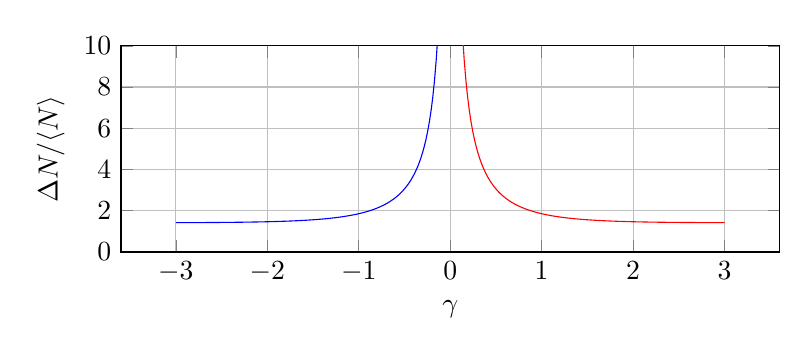
\begin{tikzpicture}
\begin{axis}[width=.82\textwidth,height=4.2cm,xlabel={$\gamma$},ylabel={$\Delta N/\langle N\rangle$},grid=major,legend style={font=\small},ymin=0,ymax=10]
\addplot+[mark=none] coordinates{(-3,1.42124195) (-2.98163522,1.42150558) (-2.96327044,1.42177912) (-2.94490566,1.42206295) (-2.92654088,1.42235746) (-2.9081761,1.42266306) (-2.88981132,1.42298015) (-2.87144654,1.42330919) (-2.85308176,1.42365061) (-2.83471698,1.4240049) (-2.8163522,1.42437253) (-2.79798742,1.42475402) (-2.77962264,1.42514989) (-2.76125786,1.42556068) (-2.74289308,1.42598697) (-2.7245283,1.42642935) (-2.70616352,1.42688842) (-2.68779874,1.42736482) (-2.66943396,1.42785922) (-2.65106918,1.42837229) (-2.6327044,1.42890475) (-2.61433962,1.42945735) (-2.59597484,1.43003084) (-2.57761006,1.43062604) (-2.55924528,1.43124377) (-2.5408805,1.43188489) (-2.52251572,1.4325503) (-2.50415094,1.43324094) (-2.48578616,1.43395777) (-2.46742138,1.4347018) (-2.4490566,1.43547407) (-2.43069182,1.43627569) (-2.41232704,1.43710776) (-2.39396226,1.43797149) (-2.37559748,1.43886808) (-2.3572327,1.4397988) (-2.33886792,1.440765) (-2.32050314,1.44176803) (-2.30213836,1.44280933) (-2.28377358,1.44389039) (-2.26540881,1.44501276) (-2.24704403,1.44617806) (-2.22867925,1.44738795) (-2.21031447,1.4486442) (-2.19194969,1.4499486) (-2.17358491,1.45130307) (-2.15522013,1.45270956) (-2.13685535,1.45417014) (-2.11849057,1.45568693) (-2.10012579,1.45726217) (-2.08176101,1.45889816) (-2.06339623,1.46059734) (-2.04503145,1.46236221) (-2.02666667,1.4641954) (-2.00830189,1.46609964) (-1.98993711,1.46807779) (-1.97157233,1.47013283) (-1.95320755,1.47226784) (-1.93484277,1.47448608) (-1.91647799,1.47679091) (-1.89811321,1.47918586) (-1.87974843,1.4816746) (-1.86138365,1.48426099) (-1.84301887,1.48694903) (-1.82465409,1.4897429) (-1.80628931,1.492647) (-1.78792453,1.49566589) (-1.76955975,1.49880435) (-1.75119497,1.5020674) (-1.73283019,1.50546026) (-1.71446541,1.50898841) (-1.69610063,1.51265758) (-1.67773585,1.51647376) (-1.65937107,1.52044325) (-1.64100629,1.52457263) (-1.62264151,1.5288688) (-1.60427673,1.533339) (-1.58591195,1.5379908) (-1.56754717,1.54283219) (-1.54918239,1.54787151) (-1.53081761,1.55311756) (-1.51245283,1.55857954) (-1.49408805,1.56426716) (-1.47572327,1.57019061) (-1.45735849,1.57636062) (-1.43899371,1.58278849) (-1.42062893,1.58948611) (-1.40226415,1.59646601) (-1.38389937,1.60374141) (-1.36553459,1.61132626) (-1.34716981,1.61923527) (-1.32880503,1.62748399) (-1.31044025,1.63608886) (-1.29207547,1.64506727) (-1.27371069,1.65443761) (-1.25534591,1.66421937) (-1.23698113,1.67443321) (-1.21861635,1.68510105) (-1.20025157,1.69624616) (-1.18188679,1.70789327) (-1.16352201,1.72006866) (-1.14515723,1.73280032) (-1.12679245,1.74611809) (-1.10842767,1.76005375) (-1.09006289,1.77464125) (-1.07169811,1.78991688) (-1.05333333,1.80591945) (-1.03496855,1.82269052) (-1.01660377,1.84027466) (-0.998238994,1.85871972) (-0.979874214,1.87807711) (-0.961509434,1.89840218) (-0.943144654,1.91975459) (-0.924779874,1.94219871) (-0.906415094,1.96580412) (-0.888050314,1.99064614) (-0.869685535,2.01680644) (-0.851320755,2.0443737) (-0.832955975,2.07344441) (-0.814591195,2.10412374) (-0.796226415,2.13652652) (-0.777861635,2.1707784) (-0.759496855,2.20701715) (-0.741132075,2.24539415) (-0.722767296,2.28607612) (-0.704402516,2.32924713) (-0.686037736,2.37511089) (-0.667672956,2.42389349) (-0.649308176,2.47584652) (-0.630943396,2.53125081) (-0.612578616,2.59042079) (-0.594213836,2.65370967) (-0.575849057,2.72151567) (-0.557484277,2.79428937) (-0.539119497,2.87254266) (-0.520754717,2.95685953) (-0.502389937,3.04790926) (-0.484025157,3.14646258) (-0.465660377,3.25341169) (-0.447295597,3.36979517) (-0.428930818,3.49682934) (-0.410566038,3.63594796) (-0.392201258,3.78885322) (-0.373836478,3.95758155) (-0.355471698,4.14459007) (-0.337106918,4.35287111) (-0.318742138,4.58610639) (-0.300377358,4.8488778) (-0.282012579,5.14696046) (-0.263647799,5.48773829) (-0.245283019,5.8808063) (-0.226918239,6.3388653) (-0.208553459,6.87908935) (-0.190188679,7.52528546) (-0.171823899,8.31143828) (-0.153459119,9.28779999) (-0.13509434,10.5319473) (-0.11672956,12.1702763) (-0.0983647799,14.4235748) (-0.08,17.7153658)};
\addplot+[mark=none] coordinates{(0.08,17.7153658) (0.0983647799,14.4235748) (0.11672956,12.1702763) (0.13509434,10.5319473) (0.153459119,9.28779999) (0.171823899,8.31143828) (0.190188679,7.52528546) (0.208553459,6.87908935) (0.226918239,6.3388653) (0.245283019,5.8808063) (0.263647799,5.48773829) (0.282012579,5.14696046) (0.300377358,4.8488778) (0.318742138,4.58610639) (0.337106918,4.35287111) (0.355471698,4.14459007) (0.373836478,3.95758155) (0.392201258,3.78885322) (0.410566038,3.63594796) (0.428930818,3.49682934) (0.447295597,3.36979517) (0.465660377,3.25341169) (0.484025157,3.14646258) (0.502389937,3.04790926) (0.520754717,2.95685953) (0.539119497,2.87254266) (0.557484277,2.79428937) (0.575849057,2.72151567) (0.594213836,2.65370967) (0.612578616,2.59042079) (0.630943396,2.53125081) (0.649308176,2.47584652) (0.667672956,2.42389349) (0.686037736,2.37511089) (0.704402516,2.32924713) (0.722767296,2.28607612) (0.741132075,2.24539415) (0.759496855,2.20701715) (0.777861635,2.1707784) (0.796226415,2.13652652) (0.814591195,2.10412374) (0.832955975,2.07344441) (0.851320755,2.0443737) (0.869685535,2.01680644) (0.888050314,1.99064614) (0.906415094,1.96580412) (0.924779874,1.94219871) (0.943144654,1.91975459) (0.961509434,1.89840218) (0.979874214,1.87807711) (0.998238994,1.85871972) (1.01660377,1.84027466) (1.03496855,1.82269052) (1.05333333,1.80591945) (1.07169811,1.78991688) (1.09006289,1.77464125) (1.10842767,1.76005375) (1.12679245,1.74611809) (1.14515723,1.73280032) (1.16352201,1.72006866) (1.18188679,1.70789327) (1.20025157,1.69624616) (1.21861635,1.68510105) (1.23698113,1.67443321) (1.25534591,1.66421937) (1.27371069,1.65443761) (1.29207547,1.64506727) (1.31044025,1.63608886) (1.32880503,1.62748399) (1.34716981,1.61923527) (1.36553459,1.61132626) (1.38389937,1.60374141) (1.40226415,1.59646601) (1.42062893,1.58948611) (1.43899371,1.58278849) (1.45735849,1.57636062) (1.47572327,1.57019061) (1.49408805,1.56426716) (1.51245283,1.55857954) (1.53081761,1.55311756) (1.54918239,1.54787151) (1.56754717,1.54283219) (1.58591195,1.5379908) (1.60427673,1.533339) (1.62264151,1.5288688) (1.64100629,1.52457263) (1.65937107,1.52044325) (1.67773585,1.51647376) (1.69610063,1.51265758) (1.71446541,1.50898841) (1.73283019,1.50546026) (1.75119497,1.5020674) (1.76955975,1.49880435) (1.78792453,1.49566589) (1.80628931,1.492647) (1.82465409,1.4897429) (1.84301887,1.48694903) (1.86138365,1.48426099) (1.87974843,1.4816746) (1.89811321,1.47918586) (1.91647799,1.47679091) (1.93484277,1.47448608) (1.95320755,1.47226784) (1.97157233,1.47013283) (1.98993711,1.46807779) (2.00830189,1.46609964) (2.02666667,1.4641954) (2.04503145,1.46236221) (2.06339623,1.46059734) (2.08176101,1.45889816) (2.10012579,1.45726217) (2.11849057,1.45568693) (2.13685535,1.45417014) (2.15522013,1.45270956) (2.17358491,1.45130307) (2.19194969,1.4499486) (2.21031447,1.4486442) (2.22867925,1.44738795) (2.24704403,1.44617806) (2.26540881,1.44501276) (2.28377358,1.44389039) (2.30213836,1.44280933) (2.32050314,1.44176803) (2.33886792,1.440765) (2.3572327,1.4397988) (2.37559748,1.43886808) (2.39396226,1.43797149) (2.41232704,1.43710776) (2.43069182,1.43627569) (2.4490566,1.43547407) (2.46742138,1.4347018) (2.48578616,1.43395777) (2.50415094,1.43324094) (2.52251572,1.4325503) (2.5408805,1.43188489) (2.55924528,1.43124377) (2.57761006,1.43062604) (2.59597484,1.43003084) (2.61433962,1.42945735) (2.6327044,1.42890475) (2.65106918,1.42837229) (2.66943396,1.42785922) (2.68779874,1.42736482) (2.70616352,1.42688842) (2.7245283,1.42642935) (2.74289308,1.42598697) (2.76125786,1.42556068) (2.77962264,1.42514989) (2.79798742,1.42475402) (2.8163522,1.42437253) (2.83471698,1.4240049) (2.85308176,1.42365061) (2.87144654,1.42330919) (2.88981132,1.42298015) (2.9081761,1.42266306) (2.92654088,1.42235746) (2.94490566,1.42206295) (2.96327044,1.42177912) (2.98163522,1.42150558) (3,1.42124195)};
\end{axis}\end{tikzpicture}\end{center}

\end{solution}
\originalsection{第4题：Maxwell与单模Hamilton算符}
\begin{exercise}
用讲义的驻波模式$\boldsymbol E=\hat xC\omega q(t)\sin kz$, $\boldsymbol B=\hat yCp(t)\cos kz/c$,$\omega=ck$, 从无源Maxwell方程推$q,p$方程, 再从模式Hamilton算符证Heisenberg方程一致.
\end{exercise}
\begin{solution}
原讲义实际在Chapter 6的Section 5.3（内部公式5.38、5.40）, 不按公式号误找Chapter 5. 在$E,cB$同单位的约定,$\nabla\cdot E=\nabla\cdot B=0$, $\nabla\times E=-\partial_tB$, $\nabla\times B=\partial_tE/c^2$. 取$y$分量的Faraday式,$C\omega kq\cos kz=-C\dot p\cos kz/c$, 得$\dot p=-\omega^2q$; Ampère式的$x$分量给$Ckp\sin kz/c=C\omega\dot q\sin kz/c^2$, 得$\dot q=p$. 腔体积$V$中原模式归一化$C=\sqrt{2/(V\epsilon_0)}$, 正弦和余弦各平方积分$V/2$, 场能$\frac{\epsilon_0}2\int(E^2+c^2B^2)\dd^3r=(p^2+\omega^2q^2)/2$. 常量$C$是能量归一化系数, 在方程中消去. 模式$H=(p^2+\omega^2q^2)/2$,$[q,p]=\ii\hbar$, Heisenberg方程同给$\dot q=p,\dot p=-\omega^2q$. 从古典场模式到算符模式的动力学相同, 量子区别在非对易及离散能量.
\end{solution}
\originalsection{第5题：左右箱与非Hermitian误写}
\begin{exercise}
对称箱分为左右两室, 只保留各室最低态$\ket L,\ket R$, 对角能量移为0, $H=\Delta(\ket L\bra R+\ket R\bra L)$, $\Delta$实. (a)求能量本征对. (b)演化任意初态$c_L\ket L+c_R\ket R$. (c)初始在右室时求左室概率. (d)若错误写成$H_{\rm bad}=\Delta\ket L\bra R$, 有何问题并检验概率守恒?
\end{exercise}
\begin{solution}
在$(L,R)$基$H=\Delta\sigma_x$, 正交态$(\ket L\pm\ket R)/\sqrt2$能量$\pm\Delta$. 设$\vartheta=\Delta t/\hbar$, $H^2=\Delta^2I$把指数分为偶、奇项, $U=I\cos\vartheta-\ii\sigma_x\sin\vartheta$. 因此两室幅为
\[
c_L(t)=c_L\cos\vartheta-\ii c_R\sin\vartheta,\qquad
c_R(t)=c_R\cos\vartheta-\ii c_L\sin\vartheta.
\]
交叉项在范数和中抵消, 总概率保持$|c_L|^2+|c_R|^2$. 初始$\ket R$时左室概率$\sin^2\vartheta$.

误写矩阵$\begin{pmatrix}0&\Delta\\0&0\end{pmatrix}$不Hermitian, 且平方为0. 指数仅$I-\ii tH_{\rm bad}/\hbar$, 从$\ket R$得到$\ket R-\ii\vartheta\ket L$, 范数平方$1+\vartheta^2$. 因而该指数不幺正. 丢掉反向隧穿项既破坏Hermitian性也破坏闭系统的概率守恒.
\end{solution}
\originalsection{第6题：限制翻转幅度}
\begin{exercise}
两态$H=-\Delta\sigma_x$,$\Delta>0$, 加一个定常$\sigma_z$项, 使初始$\ket1$的存留概率周期地在1与$p_{\min}>0$之间变. 求新项.
\end{exercise}
\begin{solution}
令新$H=-\Delta\sigma_x+\eta\sigma_z$, $\Omega=\sqrt{\Delta^2+\eta^2}$. 因$H^2=\Omega^2I$, 演化$U=I\cos(\Omega t/\hbar)-\ii H\sin(\Omega t/\hbar)/\Omega$. 从$\ket1$出发转移概率$\Delta^2\sin^2(\Omega t/\hbar)/\Omega^2$, 存留最低$\eta^2/(\Delta^2+\eta^2)$. 因而$\eta=\pm\Delta\sqrt{p_{\min}/(1-p_{\min})}$, $0<p_{\min}<1$. $p_{\min}=1$不存在有限$\eta$在保持$\Delta>0$时完全不变, 只能无穷失谐极限.
\end{solution}
